\documentclass[conference]{IEEEtran}
\IEEEoverridecommandlockouts
% The preceding line is only needed to identify funding in the first footnote. If that is unneeded, please comment it out.
\usepackage{cite}
\usepackage{amsmath,amssymb,amsfonts}
\usepackage{algorithmic}
\usepackage{graphicx}
\usepackage{textcomp}
\usepackage{xcolor}
\usepackage{hyperref}

% % Enable Dark Mode %
% \pagecolor[rgb]{0,0,0} %black
% \color[rgb]{0.5,0.5,0.5} %grey 
% % Enable Dark Mode %

\def\BibTeX{{\rm B\kern-.05em{\sc i\kern-.025em b}\kern-.08em
    T\kern-.1667em\lower.7ex\hbox{E}\kern-.125emX}}
\begin{document}

\title{Broke No More: Deep Learning for Financial Forecasting by Predicting Stock Prices in Dhaka Stock Exchange with LSTM}

\author{\IEEEauthorblockN{Md Abdullahil Kafi}
\IEEEauthorblockA{190041224} 
\textit{abdullahilkafi@iut-dhaka.edu}
\and
\IEEEauthorblockN{Tasnimul Hasnat}
\IEEEauthorblockA{190041113} 
\textit{tasnimulhasnat@iut-dhaka.edu}
\and
\IEEEauthorblockN{Abid Hasan}
\IEEEauthorblockA{190041130} 
\textit{abidhasan@iut-dhaka.edu}
}

\maketitle

\begin{abstract}
Accurately predicting stock prices is a challenging task in the field of finance, with implications for traders, investors, and analysts seeking to make informed decisions. In recent years, the emergence of recurrent neural networks (RNNs) and Long Short-Term Memory (LSTM) models has garnered attention for their potential to forecast time series data. This report focuses on utilizing RNN and LSTM approaches to predict stock market prices in the Dhaka Stock Exchange (DSE), the primary stock exchange in Bangladesh.

We employed a comprehensive methodology, encompassing data acquisition, pre-processing techniques, and the proposed RNN-LSTM forecasting model. Historical price and volume data from listed companies in the DSE are utilized to train and evaluate the predictive model. Through experimentation, performance evaluation, and comparative analysis against existing methods, the effectiveness of the RNN-LSTM model is assessed.

The findings of this study contribute to the growing body of research on financial forecasting using deep learning techniques. The results highlight the potential of RNN and LSTM models in capturing temporal dependencies and uncovering patterns in stock market data. The developed predictive model provides valuable insights to assist investors in making more informed investment decisions in the context of the Dhaka Stock Exchange.
\end{abstract}

\begin{IEEEkeywords}
Stock market prediction, Recurrent neural networks, Long Short-Term Memory, Dhaka Stock Exchange.
\end{IEEEkeywords}

\section{Introduction}
For a good and successful investment, many investors are keen on understanding the future situation of the stock market. Good and effective prediction systems for the stock market help traders, investors, and analysts by providing supportive information such as the future direction of the stock market. In recent studies, recurrent neural networks (RNN) and Long Short-Term Memory (LSTM) models have gained attention for their ability to make accurate predictions on time series datasets. These models have shown promising results in capturing temporal dependencies and patterns in sequential data.

Recurrent Neural Networks (RNN) are a class of neural networks specifically designed to handle sequential data by introducing the concept of "memory" into the network. Unlike traditional feed-forward neural networks, which process input data independently, RNNs have recurrent connections that allow information to persist across different time steps. This enables the network to capture dependencies and contextual information from previous observations in the sequence. However, standard RNNs can suffer from the "vanishing gradient" problem, which hinders their ability to learn long-term dependencies.

To overcome the limitations of standard RNNs, Long Short-Term Memory (LSTM) networks were introduced. LSTMs are a specialized variant of RNNs that incorporate memory cells and gating mechanisms to selectively retain or forget information over time. The memory cells act as an internal state that can store relevant information for extended periods, allowing LSTMs to effectively capture long-term dependencies in sequential data. The gating mechanisms, consisting of input, forget, and output gates, regulate the flow of information within the LSTM cells, enabling the network to learn and adapt to complex patterns in the data.

We tried to leverage the capabilities of RNN and LSTM approaches to predict stock market indices in the Dhaka Stock Exchange (DSE). By applying RNN and LSTM models to historical price and volume data of listed companies in the DSE, we aim to develop a robust and accurate predictive model that can assist investors in making more informed investment decisions.

In this report, we provide a comprehensive analysis of the methodology employed, encompassing data acquisition, preprocessing techniques, and the proposed RNN-LSTM forecasting model. Furthermore, we present the experimental setup, performance evaluation, and comparative analysis of our model against existing methods. The findings from this study contribute to the growing body of research on financial forecasting using RNN and LSTM models, particularly in the context of the Dhaka Stock Exchange.

\section{Related Works}
The accurate prediction of stock prices has been a subject of extensive research due to its importance in making informed investment decisions. The stock market is known for its volatility and complexity, presenting a challenging environment for forecasting. Various machine learning and deep learning algorithms have been explored to tackle this task.

Machine learning algorithms, such as Linear Regression, Support Vector Machines (SVM), and Auto-Regressive Integrated Moving Average (ARIMA), have been applied to stock price prediction with varying degrees of success. However, these traditional models often struggle to capture the complex patterns and dependencies present in stock market data. The prices of stocks are highly random and exhibit characteristics of time series models, where historical prices play a crucial role in determining future prices.

To address the limitations of traditional machine learning algorithms, deep learning paradigms have gained attention, particularly the use of Long Short-Term Memory (LSTM) networks\cite{ieee}. LSTM, a type of Recurrent Neural Network (RNN), has the ability to learn and utilize historical data to make accurate predictions. Unlike conventional RNNs, LSTM overcomes the challenge of handling long-term dependencies and the vanishing gradient problem.

The concept of LSTM revolves around capturing the context-specific dependence of stock prices on their past values. By incorporating the historical price data, trends, and patterns, LSTM models can effectively forecast stock prices. LSTM networks provide fine control over the selective forgetting and utilization of past context, making them suitable for predicting future stock prices.

One recent study proposed a Multi-Layer Sequential LSTM (MLS LSTM) model, which introduces an optimization approach for stock price forecasting. The MLS LSTM algorithm leverages the adam optimizer and employs normalized time series data divided into time steps to establish relationships between past and future values. Experimental results demonstrated its superior performance, surpassing other machine learning and deep learning algorithms with a prediction accuracy of 95.9\% on the training dataset and 98.1\% on the testing dataset\cite{sd}.

While previous studies have made significant strides in stock price prediction, further research is needed to explore the potential of deep learning algorithms and LSTM models in capturing the dynamic nature of stock markets. By understanding the context-specific dependence of stock prices on their past values, deep learning techniques offer promising avenues for improving the accuracy and reliability of stock market forecasts.

In the next section, we will present the methodology employed in this project, encompassing data acquisition, pre-processing techniques, and the proposed RNN-LSTM forecasting model.

\section{Methodology}
In this section, we outline the methodology adopted for forecasting the stock prices of companies listed on the Dhaka Stock Exchange (DSE) using deep learning with LSTM (Long Short-Term Memory) models. The methodology covers data acquisition, preprocessing, and the proposed method for predicting stock prices.

\subsection{Data Acquisition}
In Bangladesh, there are two major stock exchanges, namely the Dhaka Stock Exchange (DSE) and the Chittagong Stock Exchange (CSE). As the DSE is the larger of the two exchanges, we focused our efforts on acquiring data from this exchange.To obtain the necessary dataset for our analysis, we explored various sources of stock market data related to the Dhaka Stock Exchange.Notably, platforms such as Kaggle, a popular dataset gathering website, already host several datasets containing stock trading information for the DSE. These datasets typically include ticker information for various companies listed on the exchange, indexed by daily dates. The available data encompasses attributes such as opening price, closing price, highest price, lowest price, trading volume, and other associated parameters. However, since our primary objective is stock price prediction, we selected the relevant features that contribute to our predictive model.
While Kaggle and similar platforms provide readily available datasets, we encountered an issue with their timeliness. The available datasets were often outdated, with information spanning back several years, typically three to four years old. Consequently, we sought alternative methods to obtain more up-to-date data and decided to scrape the data directly from the official DSE website. Thankfully, we discovered existing work that had addressed this challenge by developing data scraping tools specifically for the DSE website. Leveraging one of these tools, which we found on GitHub Repository \cite{bdstockexchange}, we successfully scraped the required data from January 2008 up until December 2022.



\subsection{Data Processing}\label{AA}
The acquired dataset must undergo a series of preprocessing steps to ensure its suitability for training LSTM models. This involves handling missing values, scaling numerical features, and encoding categorical variables. In our preprocessing pipeline, we address missing values using techniques such as imputation or removal, depending on the extent of missingness and the specific requirements of the dataset. By filling in or removing missing values, we ensure that the data is complete and ready for analysis.

Furthermore, to enhance the performance of the LSTM models during training, numerical features are scaled to a consistent range. This scaling process involves methods like min-max scaling or standardization, which normalize the values to a common scale. By bringing the numerical features within a standardized range, we reduce the influence of outliers and facilitate more effective learning by the models.

In addition to handling missing values and scaling numerical features, we also consider the incorporation of categorical variables. If the dataset contains categorical variables, they need to be appropriately encoded to be utilized by the LSTM models. Common techniques for encoding categorical variables include one-hot encoding and label encoding. These methods convert categorical data into numerical representations that can be understood by the models, allowing for their integration into the forecasting process.

While the dataset provides essential information such as opening prices, closing prices, highs, and lows, these features are absolute values and may not exhibit direct correlations with the predicted stock prices. To establish meaningful relationships and enhance the predictive capabilities of the models, it is necessary to create relational data. This can be achieved through the inclusion of additional columns that capture relationships between existing features. For example, one approach we employ is to introduce a new column representing yesterday's closing price as a relational feature. By introducing such relational data, the models are provided with meaningful context and information that can potentially improve their forecasting accuracy.

Moreover, we explore various other types of relational features to evaluate their impact on the model's performance. These features may include ratios between different data fields, differences between values, or other relevant mathematical operations. By experimenting with different relational features, we aim to identify the most effective ones for our specific forecasting task.

By undertaking these preprocessing steps and incorporating relational data, we ensure that the LSTM models have the necessary information and context to make accurate predictions. This comprehensive preprocessing pipeline allows us to harness the power of deep learning and LSTM models for stock price forecasting on the Dhaka Stock Exchange.




\subsection{Core Mechanism of the Model}
Our proposed method for forecasting stock prices utilizes deep learning with LSTM models. Before we proceed further, it is  imperative to understand how this essential tool under our belt works.\\
Long Short-Term Memory (LSTM) is a type of recurrent neural network (RNN) architecture that has proven to be highly effective in time series forecasting tasks. LSTM models excel at capturing and leveraging temporal dependencies within sequential data, making them particularly well-suited for predicting future values based on historical patterns. In the context of forecasting, LSTM models can be utilized to predict various phenomena such as stock prices, weather patterns, sales figures, and more.

At the core of LSTM's effectiveness is its ability to handle the vanishing gradient problem, which is a challenge encountered in traditional RNNs. The vanishing gradient problem arises when gradients, which carry information about how the model should update its weights, diminish exponentially over time. As a result, long-term dependencies become difficult to learn, limiting the model's capacity to capture important patterns in the data. LSTM overcomes this limitation by incorporating specialized memory cells and gating mechanisms.

The LSTM architecture consists of memory cells, which act as containers to store and update information over time. Each memory cell has three essential components: an input gate, a forget gate, and an output gate. These gates regulate the flow of information within the memory cell, allowing it to selectively retain or discard information based on its relevance to the current prediction task.
Here's a detailed explanation of how LSTM works:
\begin{itemize}
  \item Input Processing: In the first step, the LSTM model receives sequential input data, which can be represented as a time series of observations. Each observation at time $t$ consists of multiple features, and the model processes these features one time step at a time.
  
  \item Information Flow: At each time step, the LSTM model takes in the current input and combines it with the information from the previous time step. The model then uses various transformations and computations to update the memory cell and generate an output for the current time step.
  
  \item Input Gate: The input gate determines how much new information should be stored in the memory cell. It takes the current input and the previous hidden state as inputs and applies a sigmoid activation function to produce an output between 0 and 1. This output represents the amount of information to be stored in the memory cell.
  
  \item Forget Gate: The forget gate decides which information from the previous memory cell state should be discarded. It takes the current input and the previous hidden state as inputs and applies a sigmoid activation function. The output of the forget gate, ranging from 0 to 1 for each memory cell component, determines the degree to which the corresponding information should be forgotten.
  
  \item Memory Update: The memory cell updates its state based on the input gate, forget gate, and the previous memory cell state. The input gate controls the amount of new information to be added to the cell, while the forget gate determines which information from the previous cell state should be erased. The updated memory cell state retains relevant information from previous steps and incorporates new information from the current input.
  
  \item Output Gate: The output gate decides how much of the memory cell state should be exposed as the output for the current time step. It takes the current input and the previous hidden state as inputs, applies a sigmoid activation function, and generates an output between 0 and 1. This output is then passed through a tanh activation function to compute the actual output value for the current time step.
  
  \item Hidden State Update: The hidden state, also known as the output of the LSTM cell, is calculated by applying the output gate to the current memory cell state. The hidden state serves as the memory of the LSTM and carries information to the next time step.
  
  \item Recursive Processing: The LSTM model repeats the above steps for each time step in the input sequence, updating the memory cell state, hidden state, and producing an output at each step.
  
  \item Training and Backpropagation: During the training process, the LSTM model learns the optimal parameters that minimize the prediction error. This is achieved by using backpropagation through time (BPTT), which is an extension of traditional backpropagation. BPTT propagates the error gradients through all the time steps, allowing the model to update its parameters based on the accumulated information from the entire sequence.
\end{itemize}

By leveraging the memory cells and gating mechanisms, LSTM models can effectively capture and learn from long-term dependencies in the input data. This makes them powerful tools for forecasting tasks where the historical context plays a crucial role in predicting future outcomes. LSTM's ability to handle sequential data and capture temporal patterns has made it a popular choice in various domains, including finance, weather forecasting, natural language processing, and more.

\subsection{Proposed Method}
LSTM models are well-suited for time series forecasting tasks such as stock price prediction due to their ability to capture and utilize temporal dependencies within sequential data. By leveraging this capability, LSTM models can effectively learn from historical stock price data and identify patterns and trends that can help predict future price movements.

To apply LSTM for stock price prediction, a common approach is to organize the data into input-output pairs. This involves creating sliding windows of a fixed length, such as 30 days or 5 days, where each window represents a sequence of past stock price observations. The target value for each window is set as the subsequent stock price value. By training the LSTM model on these input-output pairs, the model learns to recognize the underlying patterns and relationships within the data.

In the training process, the LSTM model utilizes historical stock price data to optimize its parameters. Techniques such as back-propagation and gradient descent are employed to minimize the prediction errors and improve the model's accuracy. However, to assess the model's performance and ensure its generalizability, it is crucial to evaluate it on a separate test set that contains unseen data. In this case, the month of December 2022 data can be extracted as the testing set.

Before conducting the final evaluation on the testing set, it is common practice to modify and refine the model using a validation set. The validation set is created by taking the next 1 day after each sliding window and using it as a validation sample. By analyzing the model's performance on the validation set, adjustments and enhancements can be made to improve its accuracy and predictive capabilities.

To iteratively refine the model, the sliding window is shifted by a day in each iteration. For instance, if a 5-day sliding window was initially used with days 1 to 5 as the training set and day 6 as the validation set, in the next iteration, days 2 to 6 would be used as the training set and day 7 as the validation set. This process continues throughout the entire dataset, allowing the model to learn from different segments and patterns within the data.

The accuracy of the LSTM model is ultimately assessed using the testing set, which contains the month of December 2022 data. By comparing the predicted stock prices with the actual prices in the testing set, the model's accuracy can be evaluated, and its performance can be analyzed based on relevant metrics.

In summary, the iterative process of training, validation, and testing using sliding windows allows the LSTM model to learn from historical stock price data, refine its parameters, and make accurate predictions for unseen stock price sequences.

% \subsection{Evaluation Metric}
% To evaluate the performance of the LSTM algorithm for stock price prediction, various evaluation metrics are utilized. Two commonly used metrics are Mean Squared Error (MSE) and the coefficient of determination (R-squared).

% Mean Squared Error (MSE) measures the average squared difference between the predicted stock prices and the actual prices. It provides an overall assessment of the model's accuracy by quantifying the extent of prediction errors. A lower MSE value indicates a better fit between the predicted and actual prices, implying higher accuracy in the stock price forecasts.

% The coefficient of determination, commonly denoted as R-squared, assesses the proportion of the variance in the target variable (stock prices) that can be explained by the input features. R-squared ranges between 0 and 1, with a higher value indicating a better fit of the model to the data. A higher R-squared value signifies that a larger proportion of the stock price variations can be accounted for by the input features used in the LSTM model.

% In addition to MSE and R-squared, you mentioned that a boolean value was created to determine whether or not to buy the stock. This binary metric can be used to evaluate the performance of the LSTM model in making buy/sell decisions. By comparing the predicted buy/sell recommendations with the actual decisions, you can assess the accuracy and effectiveness of the model's buy/sell predictions.

% By considering these evaluation metrics, including MSE, R-squared, and the buy/sell decision accuracy, you can comprehensively evaluate the performance of the LSTM algorithm for stock price prediction. These metrics provide insights into the accuracy of the predicted prices, the explanatory power of the input features, and the effectiveness of the model in making buy/sell recommendations.


\section{Experimental Setup}

In this section, we describe the experimental setup used to evaluate the performance of the LSTM algorithm for stock price prediction. We outline the data used, the evaluation metrics employed, and the methodology for training and testing the LSTM models.

\subsection{Data}

For our experiments, we obtained stock price data from the Dhaka Stock Exchange (DSE). The data includes daily ticker information for various companies listed on the DSE. We collected the data from January 2008 to December 2022, using a data scraping tool available on GitHub \cite{bdstockexchange}. This dataset provides us with the necessary information such as opening price, closing price, highest price, lowest price, and volume of stocks traded.

To prepare the data for training the LSTM models, we performed several preprocessing steps. This involved handling missing values, scaling numerical features, and encoding categorical variables. We employed techniques like imputation or removal for missing value handling, min-max scaling or standardization for numerical feature scaling, and appropriate encoding techniques such as one-hot encoding or label encoding for categorical variables.

\subsection{Evaluation Metrics}

To assess the performance of the LSTM models, we utilized several evaluation metrics. Firstly, we employed Mean Squared Error (MSE) to measure the average squared difference between the predicted stock prices and the actual prices. A lower MSE indicates higher accuracy in the stock price forecasts.

Additionally, we used the coefficient of determination (R-squared) to determine the proportion of variance in the target variable (stock prices) that can be explained by the input features. Higher R-squared values indicate a better fit of the model to the data, indicating more effective predictions.

Moreover, we introduced a boolean metric to evaluate the accuracy of the buy/sell recommendations made by the LSTM models. By comparing the predicted buy/sell decisions with the actual decisions, we can assess the model's performance in making accurate buy/sell predictions.




\section{Result Analysis}

Figure \ref{fig:fig1} shows the actual data that was scraped from the DSE website containing all the ticker information of all indexed stocks from January 2008 to December 2022.

\begin{figure}[htbp]
    \centering
    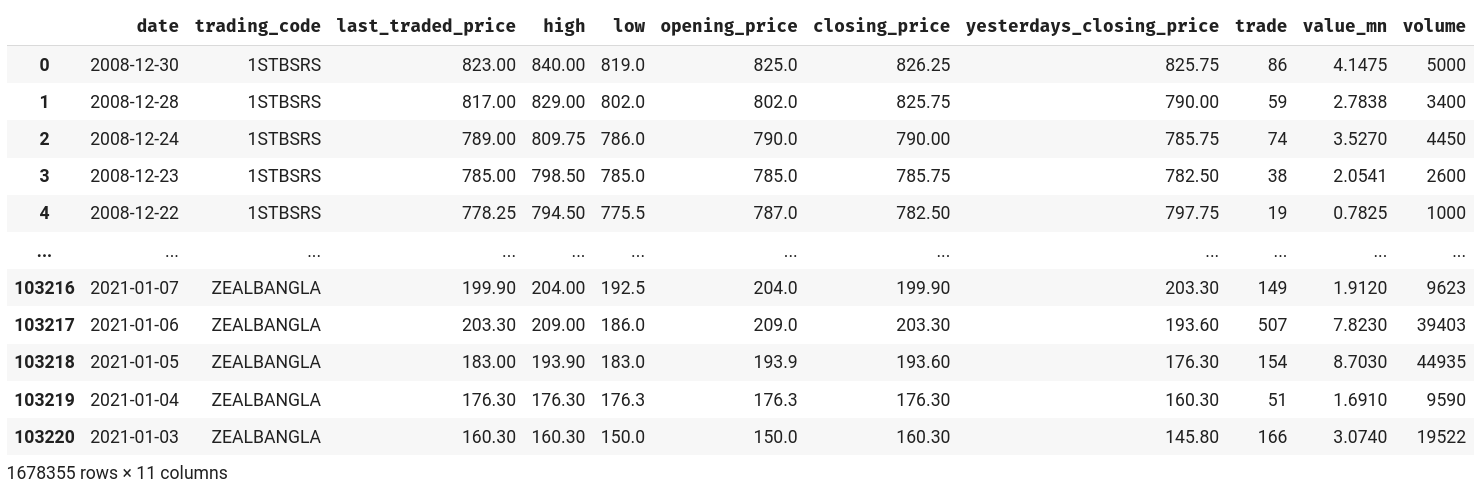
\includegraphics[width=0.975\columnwidth]{fig1.png}
    \caption{All Ticker Information}
    \label{fig:fig1}
\end{figure}

Alternately figure \ref{fig:fig2} shows only the ticker information of a particular stock, namely here AB Bank was chosen as an example.
% \subsection{Visualizations}
% In this section, we present visualizations of the predicted stock prices.

\begin{figure}[htbp]
    \centering
    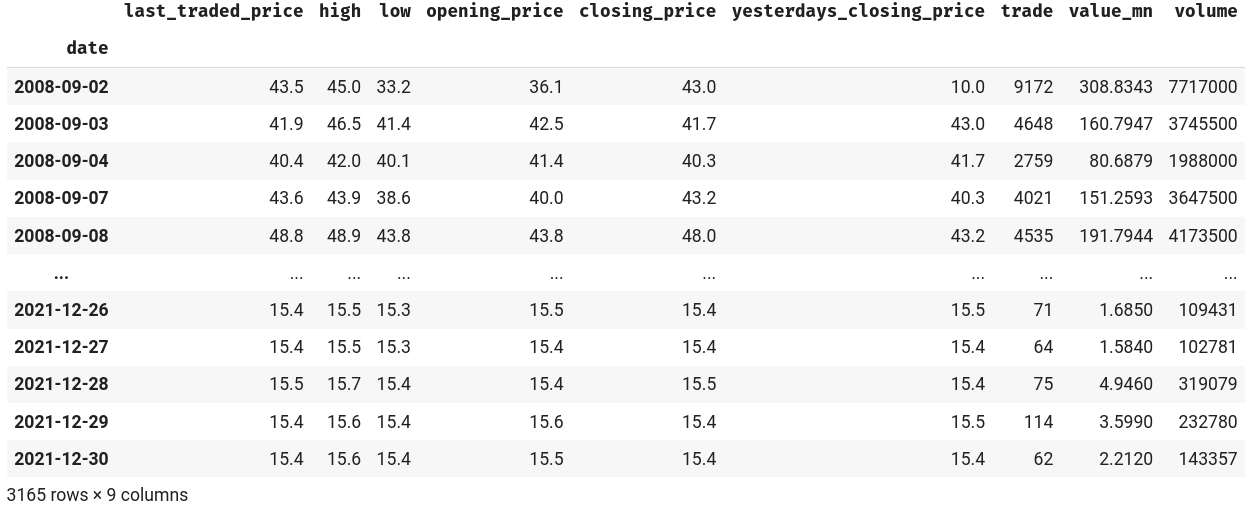
\includegraphics[width=0.975\columnwidth]{fig2.png}
    \caption{Ticker  Information of AB Bank}
    \label{fig:fig2}
\end{figure}

\begin{figure}[htbp]
    \centering
    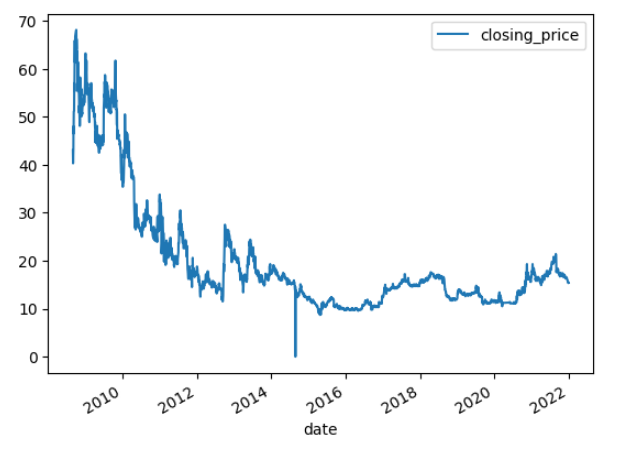
\includegraphics[width=0.975\columnwidth]{fig3.png}
    \caption{Closing Price Plotted}
    \label{fig:fig3}
\end{figure}

\begin{figure}[htbp]
    \centering
    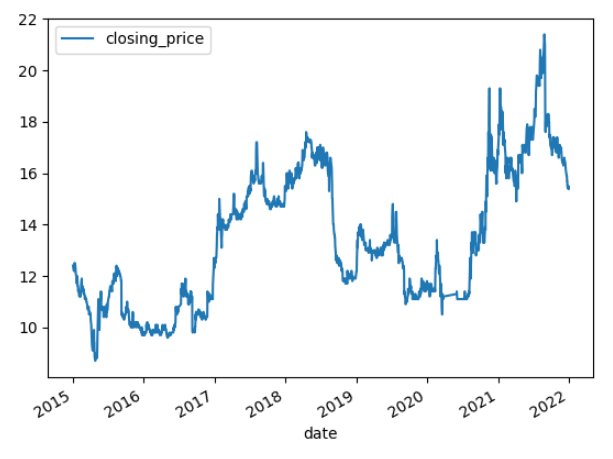
\includegraphics[width=0.975\columnwidth]{fig4.png}
    \caption{Truncated Plot of Closing Price}
    \label{fig:fig4}
\end{figure}

\begin{figure}[htbp]
    \centering
    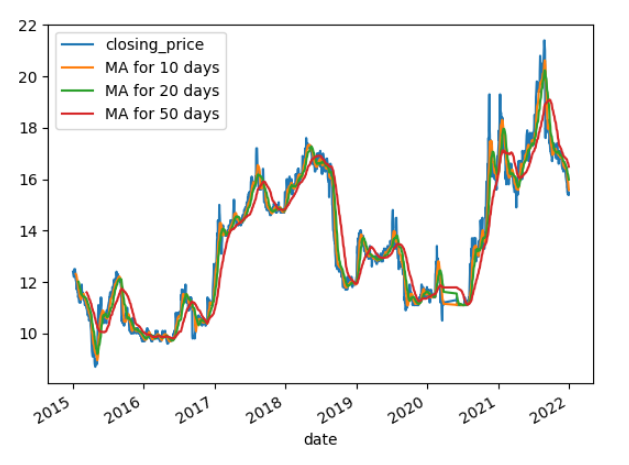
\includegraphics[width=0.975\columnwidth]{fig5.png}
    \caption{Various Moving Averages \& their correlations}
    \label{fig:fig5}
\end{figure}


\begin{figure}[htbp]
    \centering
    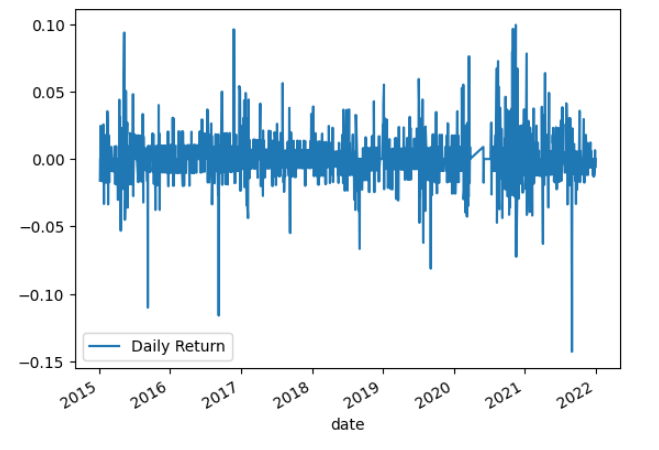
\includegraphics[width=0.975\columnwidth]{fig6.png}
    \caption{Daily Return over the time period}
    \label{fig:fig6}
\end{figure}

\begin{figure}[htbp]
    \centering
    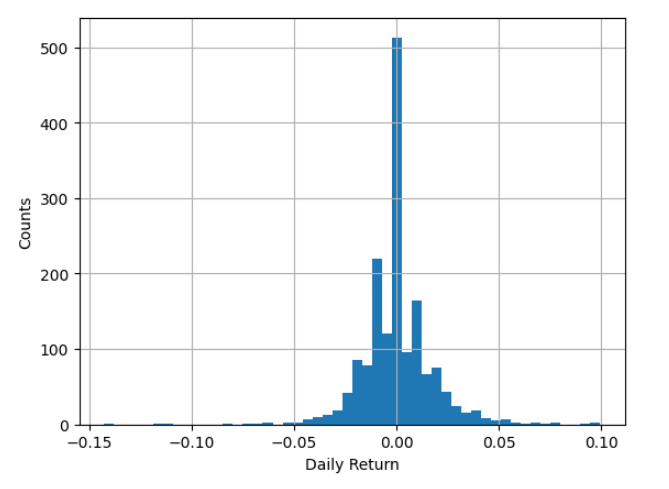
\includegraphics[width=0.975\columnwidth]{fig7.png}
    \caption{Better Visualization of Daily Return}
    \label{fig:fig7}
\end{figure}

\begin{figure}[htbp]
    \centering
    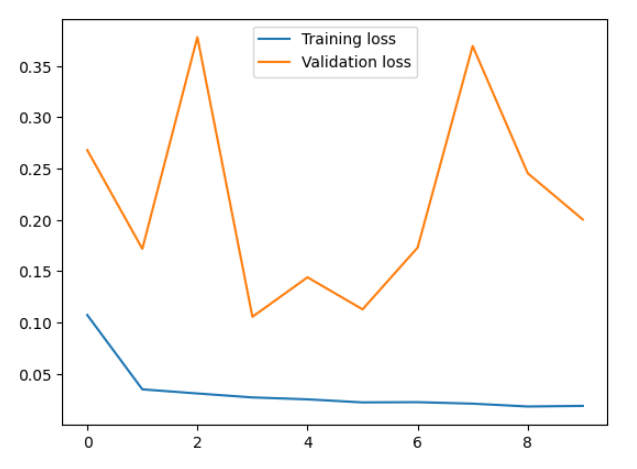
\includegraphics[width=0.975\columnwidth]{fig8.png}
    \caption{Validation Loss vs  Training Loss}
    \label{fig:fig8}
\end{figure}

% Figure \ref{fig:fig9} illustrates the performance of different LSTM models in capturing the short-term fluctuations in the stock market.

\begin{figure}[htbp]
    \centering
    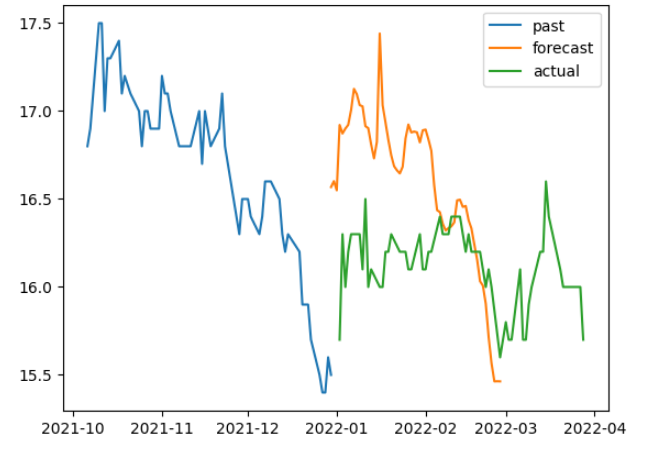
\includegraphics[width=0.975\columnwidth]{fig9.png}
    \caption{Performance of LSTM models in capturing short-term fluctuations}
    \label{fig:fig9}
\end{figure}



\section{Conclusion and Future Works}
In conclusion, our LSTM-based approach aimed to achieve improved results compared to the previous study conducted on the S\&P index fund, which achieved an accuracy of 55.9\%\cite{ieee}. However, our LSTM model did not achieve comparable results. While some companies in the Dhaka Stock Exchange (DSE) showed accuracy in the range of 60\%, others demonstrated lower accuracy levels.

Based on these findings, it may be beneficial to explore alternative tools and methodologies for stock price prediction. One promising avenue is the use of transformer models, which have gained popularity in recent years due to their effectiveness in handling sequential data\cite{trans}. Transformers utilize self-attention mechanisms to capture long-range dependencies and have shown promising results in various natural language processing and time series forecasting tasks.

Additionally, incorporating techniques like time2vec, which represents time as a continuous vector, may further enhance the forecasting capabilities on temporal data. By encoding time information in a meaningful way, time2vec can provide valuable contextual information to the model, potentially leading to more accurate predictions.

Further research and experimentation with advanced models like transformers and innovative time encoding techniques are recommended for future work. These advancements can potentially overcome the limitations observed in the LSTM-based approach and provide more accurate and reliable stock price forecasting in the context of the Dhaka Stock Exchange and other financial markets.

\begin{thebibliography}{00}
\bibitem{bdstockexchange} Code for Data Scraping, GitHub Repository. \\
\url{https://github.com/diptomondal007/bdstockexchange}

\bibitem{ieee} D. M. Q. Nelson, A. C. M. Pereira and R. A. de Oliveira, "Stock market's price movement prediction with LSTM neural networks," 2017 International Joint Conference on Neural Networks (IJCNN), Anchorage, AK, USA, 2017, pp. 1419-1426, doi: 10.1109/IJCNN.2017.7966019.
\bibitem{sd} Abdul Quadir Md, Sanjit Kapoor, Chris Junni A.V., Arun Kumar Sivaraman, Kong Fah Tee, Sabireen H., Janakiraman N.,
Novel optimization approach for stock price forecasting using multi-layered sequential LSTM,
Applied Soft Computing,
Volume 134,
2023,
109830,
ISSN 1568-4946,
https://doi.org/10.1016/j.asoc.2022.109830.
\bibitem{trans}Chaojie Wang, Yuanyuan Chen, Shuqi Zhang, and Qiuhui Zhang. 2022. 
Stock market index prediction using deep Transformer model. 
Expert Syst. Appl. 208, C (Dec 2022). 
https://doi.org/10.1016/j.eswa.2022.118128
\bibitem{collab} Project Google Collab Link 
\url{https://colab.research.google.com/drive/1kK0-O8nxK0aRfnfKoo8B-j_FxfmpgJ51?ts=648ed2b2}
\end{thebibliography}
\end{document}
